\chapter{Trusses in a nutshell}
After summarizing fundamentals of optimization in previous chapters, we can finally focus on the structural part of \emph{structural optimization}. Hence, we start with fundamentals of discrete truss structures in this chapter and optimize those in the next chapter. 


\begin{objectives}{}{objectives_sizing}
After studying this chapter and finishing the exercise, you should be able to 
\begin{itemize}[label=$\dots$]
    \item explain how general 2D truss problems can be solved employing element stiffness matrices and global stiffness matrices
    \item define your own 2D truss structures and use the accompanying code to solve them
    \item differentiate size, topology, and shape optimization of trusses
\end{itemize}
\end{objectives}

\section{General 2D trusses}
A two-dimensional truss structure is defined by a finite set of $N$ nodes 
\begin{equation}
    \mathcal{N}=\{\mathbf{x}^i \in \mathcal{R}^2, i \in [0, N-1]\}
\end{equation} and a finite set of $M$ element tuples 
\begin{equation}
    \mathcal{E} = \{(\mathbf{x}^0_j, \mathbf{x}^1_j), j \in [0, M-1]\}
\end{equation} 
connecting exactly two nodes $\mathbf{x}^0_j,  \mathbf{x}^1_j \in \mathcal{N}$ each. While $\mathcal{N}$ defines the geometry of a truss, $\mathcal{E}$ defines the topology of a truss. An example of a two-dimensional truss structure with 10 nodes and 20 elements is shown in Figure \ref{fig:truss_example}.

\begin{figure}[!htpb]
    \centering
    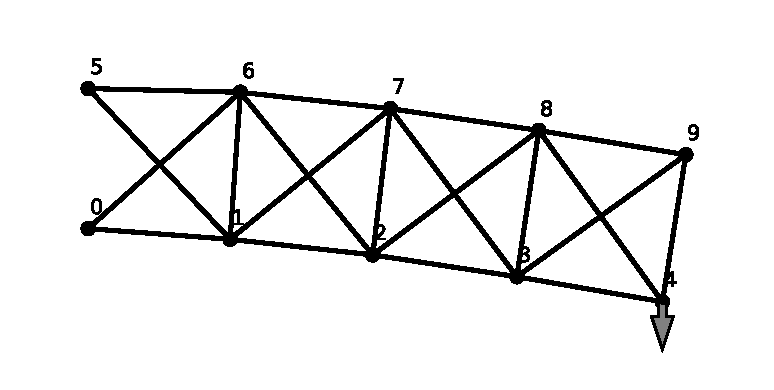
\includegraphics[width=0.75\textwidth]{figures/truss_sample.pdf}
    \caption{Example of a truss with $N=10$ numbered nodes.}
    \label{fig:truss_example}
\end{figure}

In this lecture, all elements transfer only axial forces (positive for tension, negative for compression), have a constant Young's modulus $E$, and have element-wise constant cross sectional areas $\mathbf{a} \in \mathcal{R}^M$. Each node has two degrees of freedom to deform $\mathbf{u}^i \in \mathcal{R}^2$, unless a degree of freedom is constrained by a support. The actual values of $\mathbf{u}^i$ depend on the truss design, i.e. the cross sectional areas or positions of nodes. At each node, there may also act an external force $\mathbf{f}^i \in \mathcal{R}^2$, which is independent of the truss design.

\begin{figure}[!htpb]
    \centering
    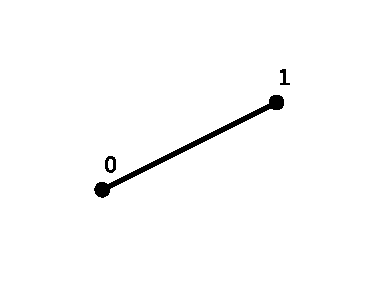
\includegraphics[width=0.4\textwidth]{figures/single_truss.pdf}
    \caption{A single truss element with two nodes.}
    \label{fig:single_truss}
\end{figure}


Without considering optimization for now, we are generally interested in solving the truss problem for the unknown displacements $\mathbf{u}^i$. To do so, we take a look at a single element, like the one shown in Figure \ref{fig:single_truss}. This truss element is defined by two nodes at positions $\mathbf{x}^0_j$ and $\mathbf{x}^1_j$. It has four degrees of freedom 
\begin{equation}
    \mathbf{u}_j = 
    \begin{pmatrix}
        \mathbf{u}^0_j \\  \mathbf{u}^1_j
    \end{pmatrix}
    = 
    \begin{pmatrix}
        (u_1)^0_j \\ (u_2)^0_j \\  (u_1)^1_j \\ (u_2)^1_j
    \end{pmatrix}
\end{equation} 
and four nodal forces 
\begin{equation}
    \mathbf{f}_j = 
    \begin{pmatrix}
        \mathbf{f}^0_j \\  \mathbf{f}^1_j
    \end{pmatrix}
    = 
    \begin{pmatrix}
        (f_1)^0_j\\ (f_2)^0_j\\ (f_1)^1_j \\ (f_2)^1_j
    \end{pmatrix},
\end{equation} 
where $\mathbf{u}_j \in \mathcal{R}^4$ and $\mathbf{f}_j \in \mathcal{R}^4$. 
The displacements can be related to the nodal forces via 
\begin{equation}
    \mathbf{f}_j = \mathbf{k}_j \cdot \mathbf{u}_j
    \label{eq:local_truss_stiffness}
\end{equation}
with an element stiffness matrix $\mathbf{k}_j \in \mathcal{R}^{4\times4}$ defined as \cite{Christensen2008}
\begin{equation}
    \mathbf{k}_j = \frac{a_j E}{l_j}
    \begin{pmatrix}
    \cos{\phi}^2 & \cos{\phi}\sin{\phi} & -\cos{\phi}^2 & -\cos{\phi}\sin{\phi} \\
    \cos{\phi}\sin{\phi} & \sin{\phi}^2 & -\cos{\phi}\sin{\phi} & -\sin{\phi}^2 \\
    -\cos{\phi}^2 & \cos{\phi}\sin{\phi} & \cos{\phi}^2 &\cos{\phi}\sin{\phi} \\
    -\cos{\phi}\sin{\phi} & -\sin{\phi}^2 & \cos{\phi}\sin{\phi} & \sin{\phi}^2 \\
    \end{pmatrix}
\end{equation}
using the orientation angle of the element $\phi = \arctan\left(\frac{x^0_2-x^1_2}{x^0_1-x^1_1}\right)$, the cross sectional area of an element $a_j$, and the length 
\begin{equation}
    l_j = \sqrt{(x^0_2-x^1_2)^2 + (x^0_1-x^1_1)^2}.
\end{equation}
This element stiffness matrix is symmetric and positive semi-definite, i.e. \begin{equation}
    \mathbf{v} \cdot \mathbf{k}_j \cdot \mathbf{v} \ge 0 \hspace{0.5em} \forall \mathbf{v}.
\end{equation}

Similar to the local relation in Equation \eqref{eq:local_truss_stiffness}, we can denote a global relation for all degrees of freedom $\mathbf{u} \in \mathcal{R}^{2N}$ and all forces $\mathbf{f} \in \mathcal{R}^{2N}$ as 
\begin{equation}
    \mathbf{f} = \mathbf{K} \cdot  \mathbf{u} 
    \label{eq:global_stiffness}
\end{equation}
with a global stiffness matrix $\mathbf{K} \in \mathcal{R}^{2N \times 2N}$. This global stiffness matrix is \emph{assembled} from element stiffness matrices by adding entries of all element stiffness matrices at the correct positions. This can be written as 
\begin{equation}
    \underbrace{
    \begin{pmatrix}
        \dots \\ (f_1)^0_j \\ (f_2)^0_j \\ \dots \\ (f_1)^1_j \\ (f_2)^1_j \\ \dots \\
    \end{pmatrix}}_{\mathbf{f}}
    =
    \underbrace{
    \sum_j
    \underbrace{
    \begin{pmatrix}
    \dots & \dots & \dots & \dots & \dots & \dots & \dots \\
    \dots & (k_{11})_j & (k_{12})_j & \dots & (k_{13})_j & (k_{14})_j & \dots  \\
    \dots & (k_{21})_j & (k_{22})_j & \dots & (k_{23})_j & (k_{24})_j & \dots  \\
    \dots & \dots & \dots & \dots & \dots & \dots & \dots  \\
    \dots & (k_{31})_j & (k_{32})_j & \dots & (k_{33})_j & (k_{34})_j & \dots  \\
    \dots & (k_{41})_j & (k_{42})_j & \dots & (k_{43})_j & (k_{44})_j & \dots  \\
    \dots & \dots & \dots & \dots & \dots & \dots & \dots  \\
    \end{pmatrix}}_{\mathbf{K}_j}
    }_{\mathbf{K}}
    \underbrace{
    \begin{pmatrix}
        \dots \\ (u_1)^0_j \\ (u_2)^0_j \\ \dots \\ (u_1)^1_j \\ (u_2)^1_j \\ \dots \\
    \end{pmatrix}}_{\mathbf{u} (\mathbf{a})},
\end{equation}
where the degrees of freedom $(u_1)^0_j, (u_2)^0_j$ etc. are at the positions in the vector corresponding to the global node displacements $\mathbf{u}$. The matrices $\mathbf{K}_j$ are zero everywhere except for the 16 positions at which they are filled with values from $\mathbf{k}_j$.
The global stiffness matrix is symmetric and positive semi-definite, just like the element stiffness matrix.

Before solving the global system of equations, we need to remove those entries containing constrained degrees of freedom. This is achieved by simply removing all constrained entries in $\mathbf{f}$ and $\mathbf{u}$ and the corresponding rows and columns in the global stiffness matrix $\mathbf{K}$. If we do not remove sufficient degrees of freedom, the matrix would be singular and cannot be solved. The physical interpretation of this behavior is simple: The truss would be statically undetermined and can experience rigid body motions.

Finally, after removing constraints, we end up with a reduced system of equations 
\begin{equation}
     \mathbf{f}_\textrm{red} = \mathbf{K}_\textrm{red}  \cdot \mathbf{u}_\textrm{red} 
     \label{eq:reduced_system}
\end{equation}
where $\mathbf{K}_\textrm{red}$ is strictly positive definite and not singular (if sufficient boundary conditions have been applied). Solving this system of equation gives us the unknown node displacements $\mathbf{u}$. 

\begin{figure}[!htpb]
    \centering
    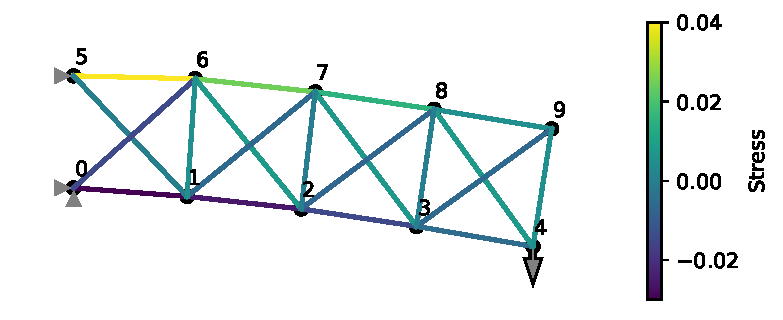
\includegraphics[width=\textwidth]{figures/truss_sample_solved.pdf}
    \caption{Exemplary solution of a truss computation for the example shown in Figure \ref{fig:truss_example}.}
    \label{fig:truss_example_solved}
\end{figure}

As a post-processing step, we may compute the stress in each element via
\begin{equation}
    S_j = \frac{E}{l_j} 
    \begin{pmatrix}
        \cos{\phi} & \sin{\phi} & -\cos{\phi} & -\sin{\phi}
    \end{pmatrix}
    \cdot 
    \mathbf{u}_j.
\end{equation}

An exemplary solution for the example shown in Figure \ref{fig:truss_example} is given in Figure \ref{fig:truss_example_solved} with colors indicating the stresses in trusses.

\begin{example}{Three bar truss}{trussexample}
    Consider the truss shown below, which is subjected to a force $P$ indicated by the gray arrow and supports indicated by gray triangles. It has three nodes 
    \begin{equation}
        \mathcal{N} = \{\mathbf{x}^0=(1,0)^\top, \mathbf{x}^1=(0,0)^\top,\mathbf{x}^2=(0,1)^\top \}
    \end{equation}
    and three elements 
    \begin{equation}
        \mathcal{E} = \{(\mathbf{x}^0, \mathbf{x}^1), (\mathbf{x}^0, \mathbf{x}^2), (\mathbf{x}^1, \mathbf{x}^2)\}.
    \end{equation}

    \begin{center}
        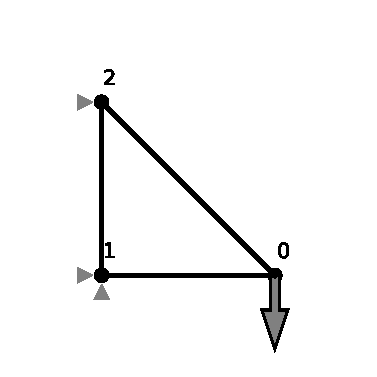
\includegraphics[width=0.5\textwidth]{figures/three_bar_truss.pdf}
    \end{center}

    The element stiffness matrices in local coordinates are 
    \begin{equation}
        \mathbf{k}_0 = E a_0
        \begin{pmatrix}
             1 & 0 & -1 & 0 \\
             0 & 0 &  0 & 0 \\
            -1 & 0 &  1 & 0 \\
             0 & 0 &  0 & 0
        \end{pmatrix},
    \end{equation}
    \begin{equation}
        \mathbf{k}_1 = \frac{E a_1}{2\sqrt{2}}
        \begin{pmatrix}
             1 & -1 & -1 &  1 \\
            -1 &  1 &  1 & -1 \\
            -1 &  1 &  1 & -1 \\
             1 & -1 & -1 &  1
        \end{pmatrix}
    \end{equation}
    and 
    \begin{equation}
        \mathbf{k}_2 = E a_2
        \begin{pmatrix}
            0 &  0 & 0 &  0 \\
            0 &  1 & 0 & -1 \\
            0 &  0 & 0 &  0 \\
            0 & -1 & 0 &  1 
        \end{pmatrix}.
    \end{equation}

    The global stiffness matrix is 
    \begin{equation}
        \mathbf{K} = E
        \begin{pmatrix}
             a_0 + \frac{a_1}{2\sqrt{2}}&  -\frac{a_1}{2\sqrt{2}} & \cellcolor{aux_green!10}-a_0 &  \cellcolor{aux_green!10}0 & -\cellcolor{aux_green!10} \frac{a_1}{2\sqrt{2}} &  \frac{a_1}{2\sqrt{2}}\\
            -\frac{a_1}{2\sqrt{2}} &  \frac{a_1}{2\sqrt{2}} & \cellcolor{aux_green!10} 0 & \cellcolor{aux_green!10} 0 & \cellcolor{aux_green!10}\frac{a_1}{2\sqrt{2}} &  -\frac{a_1}{2\sqrt{2}} \\
            \rowcolor{aux_green!10}
             -a_0 &  a_0 & 0 &  0 & 0 & 0\\
             \rowcolor{aux_green!10}
            0 &  0 & 0 &  a_2 & 0 &  -a_2 \\
            \rowcolor{aux_green!10}
             -\frac{a_1}{2\sqrt{2}} &  \frac{a_1}{2\sqrt{2}} & 0 &  0 & \frac{a_1}{2\sqrt{2}} &  -\frac{a_1}{2\sqrt{2}}\\
            \frac{a_1}{2\sqrt{2}} &  -\frac{a_1}{2\sqrt{2}} & \cellcolor{aux_green!10} 0 &  \cellcolor{aux_green!10} -a_2 & \cellcolor{aux_green!10} -\frac{a_1}{2\sqrt{2}} &  a_2 + \frac{a_1}{2\sqrt{2}}\\
        \end{pmatrix}
    \end{equation}
    with colored rows and columns indicating those entries which will be removed due to constraints. This leads to the reduced system 
    \begin{equation}
        \begin{pmatrix}
            0 \\ -P \\ 0  \\
        \end{pmatrix}
         = E
        \begin{pmatrix}
             a_0 + \frac{a_1}{2\sqrt{2}}&  -\frac{a_1}{2\sqrt{2}} &  \frac{a_1}{2\sqrt{2}}\\
            -\frac{a_1}{2\sqrt{2}} &  \frac{a_1}{2\sqrt{2}} &  -\frac{a_1}{2\sqrt{2}} \\
            \frac{a_1}{2\sqrt{2}} &  -\frac{a_1}{2\sqrt{2}} &  a_2 + \frac{a_1}{2\sqrt{2}}
        \end{pmatrix}
        \mathbf{u}_\textrm{red}
    \end{equation}
    which can be solved for 
    \begin{equation}
        \mathbf{u}_\textrm{red} = 
        \begin{pmatrix}
            -\frac{P}{Ea_0} \\  \frac{2\sqrt{2}P}{Ea_2} - \frac{P}{Ea_0} - \frac{P}{Ea_1} \\ -\frac{P}{Ea_1}  \\
        \end{pmatrix}
    \end{equation}

    The final result of the computation is shown below.
    
    \begin{center}
        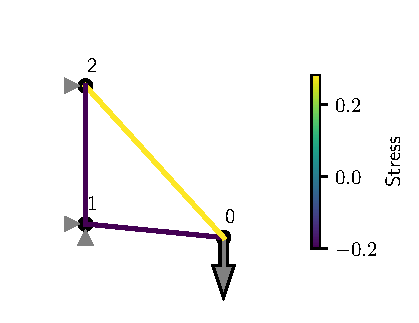
\includegraphics[width=0.5\textwidth]{figures/three_bar_truss_solved.pdf}
    \end{center}    
\end{example}

\section{Optimization types for trusses}
Truss structures may be optimized by size optimization, topology optimization and shape optimization: 
\begin{description}
    \item[Size:]{In size optimization, we seek the optimal truss cross section areas $\mathbf{a}$ for fixed node positions $\mathbf{x}$ and a fixed topology, i.e. fixed connections $\mathcal{E}$. An example for this is shown in Figure \ref{fig:bridge_size}.} 
    \item[Topology:]{In topology optimization, we want find the optimal connections in a truss $\mathcal{E}$ with cross sectional areas being either the maximum or minimum value for fixed node positions $\mathbf{x}$. An example for this is shown in Figure \ref{fig:bridge_topology}.}
    \item[Shape:]{In shape optimization, we want to find the optimal positions of nodes $\mathbf{x}$ in a truss for fixed cross sectional areas $\mathbf{a}$ and a fixed topology $\mathcal{E}$.}
\end{description}

\begin{figure}[!ht]
    \centering
    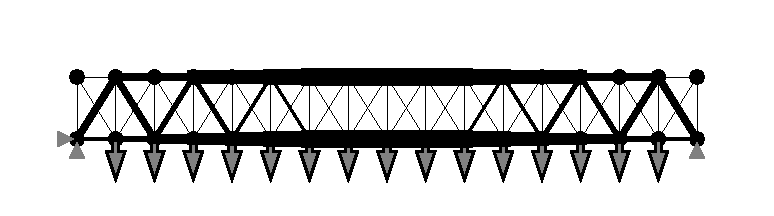
\includegraphics[width=\textwidth]{figures/bridge_size_optimized.pdf}
    \caption{Bridge truss size optimization}
    \label{fig:bridge_size}
\end{figure}

\begin{figure}[!ht]
    \centering
    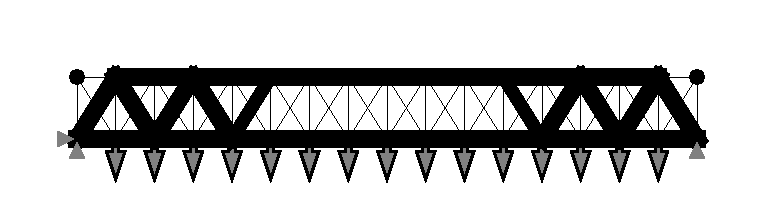
\includegraphics[width=\textwidth]{figures/bridge_topology_optimized.pdf}
    \caption{Bridge truss topology optimization}
    \label{fig:bridge_topology}
\end{figure}

\begin{figure}[!ht]
    \centering
    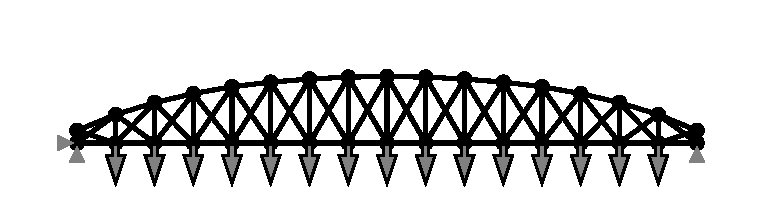
\includegraphics[width=\textwidth]{figures/bridge_shape_optimized.pdf}
    \caption{Bridge truss shape optimization}
    \label{fig:bridge_shape}
\end{figure}




\bibliographystyle{unsrtnat}
\bibliography{literature} 